% Created by tikzDevice version 0.12.6 on 2024-10-31 12:54:24
% !TEX encoding = UTF-8 Unicode
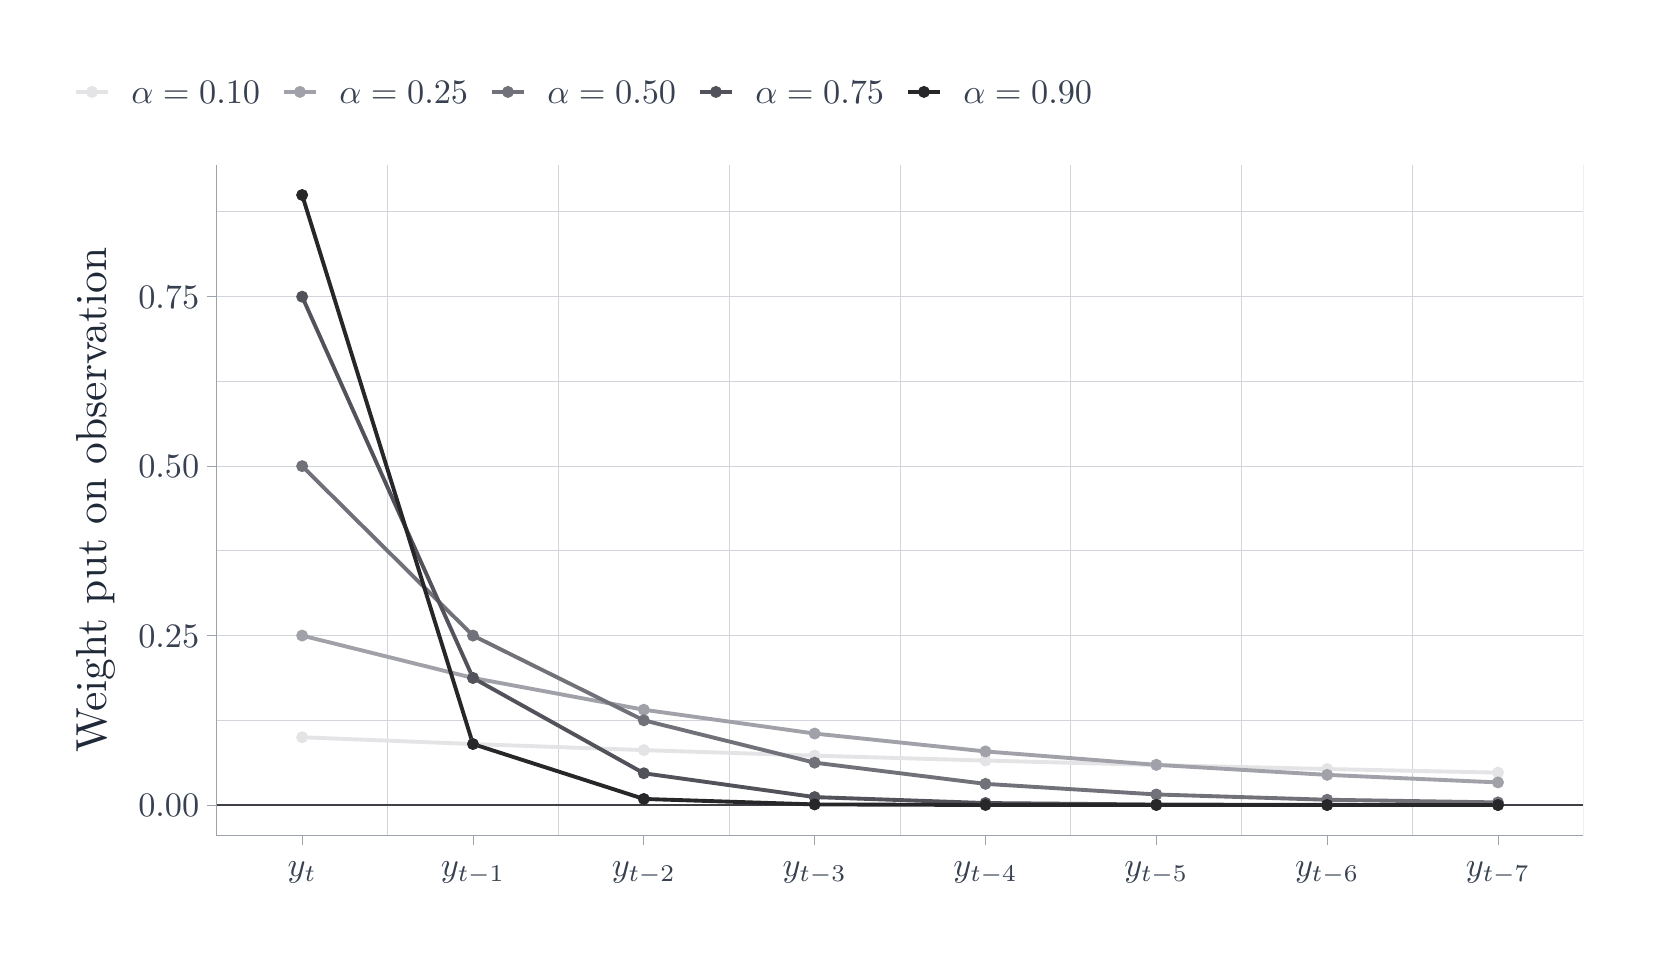
\begin{tikzpicture}[x=1pt,y=1pt]
\definecolor{fillColor}{RGB}{255,255,255}
\path[use as bounding box,fill=fillColor] (0,0) rectangle (578.16,325.21);
\begin{scope}
\path[clip] (  0.00,  0.00) rectangle (578.16,325.21);
\definecolor{drawColor}{RGB}{255,255,255}

\path[draw=drawColor,line width= 0.7pt,line join=round,line cap=round,fill=fillColor] (  0.00,  0.00) rectangle (578.16,325.21);
\end{scope}
\begin{scope}
\path[clip] ( 68.32, 33.29) rectangle (562.16,275.76);
\definecolor{drawColor}{RGB}{255,255,255}
\definecolor{fillColor}{RGB}{255,255,255}

\path[draw=drawColor,line width= 0.7pt,line join=round,line cap=round,fill=fillColor] ( 68.32, 33.29) rectangle (562.16,275.76);
\definecolor{drawColor}{RGB}{209,213,219}

\path[draw=drawColor,line width= 0.4pt,line join=round] ( 68.32, 74.92) --
	(562.16, 74.92);

\path[draw=drawColor,line width= 0.4pt,line join=round] ( 68.32,136.15) --
	(562.16,136.15);

\path[draw=drawColor,line width= 0.4pt,line join=round] ( 68.32,197.39) --
	(562.16,197.39);

\path[draw=drawColor,line width= 0.4pt,line join=round] ( 68.32,258.62) --
	(562.16,258.62);

\path[draw=drawColor,line width= 0.4pt,line join=round] ( 68.32, 33.29) --
	( 68.32,275.76);

\path[draw=drawColor,line width= 0.4pt,line join=round] (130.05, 33.29) --
	(130.05,275.76);

\path[draw=drawColor,line width= 0.4pt,line join=round] (191.78, 33.29) --
	(191.78,275.76);

\path[draw=drawColor,line width= 0.4pt,line join=round] (253.51, 33.29) --
	(253.51,275.76);

\path[draw=drawColor,line width= 0.4pt,line join=round] (315.24, 33.29) --
	(315.24,275.76);

\path[draw=drawColor,line width= 0.4pt,line join=round] (376.97, 33.29) --
	(376.97,275.76);

\path[draw=drawColor,line width= 0.4pt,line join=round] (438.70, 33.29) --
	(438.70,275.76);

\path[draw=drawColor,line width= 0.4pt,line join=round] (500.43, 33.29) --
	(500.43,275.76);

\path[draw=drawColor,line width= 0.4pt,line join=round] (562.16, 33.29) --
	(562.16,275.76);

\path[draw=drawColor,line width= 0.4pt,line join=round] ( 68.32, 44.31) --
	(562.16, 44.31);

\path[draw=drawColor,line width= 0.4pt,line join=round] ( 68.32,105.54) --
	(562.16,105.54);

\path[draw=drawColor,line width= 0.4pt,line join=round] ( 68.32,166.77) --
	(562.16,166.77);

\path[draw=drawColor,line width= 0.4pt,line join=round] ( 68.32,228.00) --
	(562.16,228.00);
\definecolor{drawColor}{RGB}{63,63,70}

\path[draw=drawColor,line width= 0.6pt,line join=round] ( 68.32, 44.31) -- (562.16, 44.31);
\definecolor{drawColor}{RGB}{228,228,231}

\path[draw=drawColor,line width= 1.4pt,line join=round] ( 99.18, 68.80) --
	(160.91, 66.35) --
	(222.64, 64.15) --
	(284.37, 62.16) --
	(346.10, 60.38) --
	(407.83, 58.77) --
	(469.56, 57.32) --
	(531.29, 56.02);
\definecolor{drawColor}{RGB}{161,161,170}

\path[draw=drawColor,line width= 1.4pt,line join=round] ( 99.18,105.54) --
	(160.91, 90.23) --
	(222.64, 78.75) --
	(284.37, 70.14) --
	(346.10, 63.68) --
	(407.83, 58.84) --
	(469.56, 55.21) --
	(531.29, 52.48);
\definecolor{drawColor}{RGB}{113,113,122}

\path[draw=drawColor,line width= 1.4pt,line join=round] ( 99.18,166.77) --
	(160.91,105.54) --
	(222.64, 74.92) --
	(284.37, 59.62) --
	(346.10, 51.96) --
	(407.83, 48.13) --
	(469.56, 46.22) --
	(531.29, 45.26);
\definecolor{drawColor}{RGB}{82,82,91}

\path[draw=drawColor,line width= 1.4pt,line join=round] ( 99.18,228.00) --
	(160.91, 90.23) --
	(222.64, 55.79) --
	(284.37, 47.18) --
	(346.10, 45.03) --
	(407.83, 44.49) --
	(469.56, 44.35) --
	(531.29, 44.32);
\definecolor{drawColor}{RGB}{39,39,42}

\path[draw=drawColor,line width= 1.4pt,line join=round] ( 99.18,264.74) --
	(160.91, 66.35) --
	(222.64, 46.51) --
	(284.37, 44.53) --
	(346.10, 44.33) --
	(407.83, 44.31) --
	(469.56, 44.31) --
	(531.29, 44.31);
\definecolor{drawColor}{RGB}{228,228,231}
\definecolor{fillColor}{RGB}{228,228,231}

\path[draw=drawColor,line width= 0.4pt,line join=round,line cap=round,fill=fillColor] ( 99.18, 68.80) circle (  1.96);

\path[draw=drawColor,line width= 0.4pt,line join=round,line cap=round,fill=fillColor] (160.91, 66.35) circle (  1.96);

\path[draw=drawColor,line width= 0.4pt,line join=round,line cap=round,fill=fillColor] (222.64, 64.15) circle (  1.96);

\path[draw=drawColor,line width= 0.4pt,line join=round,line cap=round,fill=fillColor] (284.37, 62.16) circle (  1.96);

\path[draw=drawColor,line width= 0.4pt,line join=round,line cap=round,fill=fillColor] (346.10, 60.38) circle (  1.96);

\path[draw=drawColor,line width= 0.4pt,line join=round,line cap=round,fill=fillColor] (407.83, 58.77) circle (  1.96);

\path[draw=drawColor,line width= 0.4pt,line join=round,line cap=round,fill=fillColor] (469.56, 57.32) circle (  1.96);

\path[draw=drawColor,line width= 0.4pt,line join=round,line cap=round,fill=fillColor] (531.29, 56.02) circle (  1.96);
\definecolor{drawColor}{RGB}{161,161,170}
\definecolor{fillColor}{RGB}{161,161,170}

\path[draw=drawColor,line width= 0.4pt,line join=round,line cap=round,fill=fillColor] ( 99.18,105.54) circle (  1.96);

\path[draw=drawColor,line width= 0.4pt,line join=round,line cap=round,fill=fillColor] (160.91, 90.23) circle (  1.96);

\path[draw=drawColor,line width= 0.4pt,line join=round,line cap=round,fill=fillColor] (222.64, 78.75) circle (  1.96);

\path[draw=drawColor,line width= 0.4pt,line join=round,line cap=round,fill=fillColor] (284.37, 70.14) circle (  1.96);

\path[draw=drawColor,line width= 0.4pt,line join=round,line cap=round,fill=fillColor] (346.10, 63.68) circle (  1.96);

\path[draw=drawColor,line width= 0.4pt,line join=round,line cap=round,fill=fillColor] (407.83, 58.84) circle (  1.96);

\path[draw=drawColor,line width= 0.4pt,line join=round,line cap=round,fill=fillColor] (469.56, 55.21) circle (  1.96);

\path[draw=drawColor,line width= 0.4pt,line join=round,line cap=round,fill=fillColor] (531.29, 52.48) circle (  1.96);
\definecolor{drawColor}{RGB}{113,113,122}
\definecolor{fillColor}{RGB}{113,113,122}

\path[draw=drawColor,line width= 0.4pt,line join=round,line cap=round,fill=fillColor] ( 99.18,166.77) circle (  1.96);

\path[draw=drawColor,line width= 0.4pt,line join=round,line cap=round,fill=fillColor] (160.91,105.54) circle (  1.96);

\path[draw=drawColor,line width= 0.4pt,line join=round,line cap=round,fill=fillColor] (222.64, 74.92) circle (  1.96);

\path[draw=drawColor,line width= 0.4pt,line join=round,line cap=round,fill=fillColor] (284.37, 59.62) circle (  1.96);

\path[draw=drawColor,line width= 0.4pt,line join=round,line cap=round,fill=fillColor] (346.10, 51.96) circle (  1.96);

\path[draw=drawColor,line width= 0.4pt,line join=round,line cap=round,fill=fillColor] (407.83, 48.13) circle (  1.96);

\path[draw=drawColor,line width= 0.4pt,line join=round,line cap=round,fill=fillColor] (469.56, 46.22) circle (  1.96);

\path[draw=drawColor,line width= 0.4pt,line join=round,line cap=round,fill=fillColor] (531.29, 45.26) circle (  1.96);
\definecolor{drawColor}{RGB}{82,82,91}
\definecolor{fillColor}{RGB}{82,82,91}

\path[draw=drawColor,line width= 0.4pt,line join=round,line cap=round,fill=fillColor] ( 99.18,228.00) circle (  1.96);

\path[draw=drawColor,line width= 0.4pt,line join=round,line cap=round,fill=fillColor] (160.91, 90.23) circle (  1.96);

\path[draw=drawColor,line width= 0.4pt,line join=round,line cap=round,fill=fillColor] (222.64, 55.79) circle (  1.96);

\path[draw=drawColor,line width= 0.4pt,line join=round,line cap=round,fill=fillColor] (284.37, 47.18) circle (  1.96);

\path[draw=drawColor,line width= 0.4pt,line join=round,line cap=round,fill=fillColor] (346.10, 45.03) circle (  1.96);

\path[draw=drawColor,line width= 0.4pt,line join=round,line cap=round,fill=fillColor] (407.83, 44.49) circle (  1.96);

\path[draw=drawColor,line width= 0.4pt,line join=round,line cap=round,fill=fillColor] (469.56, 44.35) circle (  1.96);

\path[draw=drawColor,line width= 0.4pt,line join=round,line cap=round,fill=fillColor] (531.29, 44.32) circle (  1.96);
\definecolor{drawColor}{RGB}{39,39,42}
\definecolor{fillColor}{RGB}{39,39,42}

\path[draw=drawColor,line width= 0.4pt,line join=round,line cap=round,fill=fillColor] ( 99.18,264.74) circle (  1.96);

\path[draw=drawColor,line width= 0.4pt,line join=round,line cap=round,fill=fillColor] (160.91, 66.35) circle (  1.96);

\path[draw=drawColor,line width= 0.4pt,line join=round,line cap=round,fill=fillColor] (222.64, 46.51) circle (  1.96);

\path[draw=drawColor,line width= 0.4pt,line join=round,line cap=round,fill=fillColor] (284.37, 44.53) circle (  1.96);

\path[draw=drawColor,line width= 0.4pt,line join=round,line cap=round,fill=fillColor] (346.10, 44.33) circle (  1.96);

\path[draw=drawColor,line width= 0.4pt,line join=round,line cap=round,fill=fillColor] (407.83, 44.31) circle (  1.96);

\path[draw=drawColor,line width= 0.4pt,line join=round,line cap=round,fill=fillColor] (469.56, 44.31) circle (  1.96);

\path[draw=drawColor,line width= 0.4pt,line join=round,line cap=round,fill=fillColor] (531.29, 44.31) circle (  1.96);
\end{scope}
\begin{scope}
\path[clip] (  0.00,  0.00) rectangle (578.16,325.21);
\definecolor{drawColor}{RGB}{156,163,175}

\path[draw=drawColor,line width= 0.3pt,line join=round] ( 68.32, 33.29) --
	( 68.32,275.76);
\end{scope}
\begin{scope}
\path[clip] (  0.00,  0.00) rectangle (578.16,325.21);
\definecolor{drawColor}{RGB}{55,65,81}

\node[text=drawColor,anchor=base east,inner sep=0pt, outer sep=0pt, scale=  1.24] at ( 62.02, 40.02) {0.00};

\node[text=drawColor,anchor=base east,inner sep=0pt, outer sep=0pt, scale=  1.24] at ( 62.02,101.25) {0.25};

\node[text=drawColor,anchor=base east,inner sep=0pt, outer sep=0pt, scale=  1.24] at ( 62.02,162.49) {0.50};

\node[text=drawColor,anchor=base east,inner sep=0pt, outer sep=0pt, scale=  1.24] at ( 62.02,223.72) {0.75};
\end{scope}
\begin{scope}
\path[clip] (  0.00,  0.00) rectangle (578.16,325.21);
\definecolor{drawColor}{RGB}{156,163,175}

\path[draw=drawColor,line width= 0.3pt,line join=round] ( 64.82, 44.31) --
	( 68.32, 44.31);

\path[draw=drawColor,line width= 0.3pt,line join=round] ( 64.82,105.54) --
	( 68.32,105.54);

\path[draw=drawColor,line width= 0.3pt,line join=round] ( 64.82,166.77) --
	( 68.32,166.77);

\path[draw=drawColor,line width= 0.3pt,line join=round] ( 64.82,228.00) --
	( 68.32,228.00);
\end{scope}
\begin{scope}
\path[clip] (  0.00,  0.00) rectangle (578.16,325.21);
\definecolor{drawColor}{RGB}{156,163,175}

\path[draw=drawColor,line width= 0.3pt,line join=round] ( 68.32, 33.29) --
	(562.16, 33.29);
\end{scope}
\begin{scope}
\path[clip] (  0.00,  0.00) rectangle (578.16,325.21);
\definecolor{drawColor}{RGB}{156,163,175}

\path[draw=drawColor,line width= 0.3pt,line join=round] ( 99.18, 29.79) --
	( 99.18, 33.29);

\path[draw=drawColor,line width= 0.3pt,line join=round] (160.91, 29.79) --
	(160.91, 33.29);

\path[draw=drawColor,line width= 0.3pt,line join=round] (222.64, 29.79) --
	(222.64, 33.29);

\path[draw=drawColor,line width= 0.3pt,line join=round] (284.37, 29.79) --
	(284.37, 33.29);

\path[draw=drawColor,line width= 0.3pt,line join=round] (346.10, 29.79) --
	(346.10, 33.29);

\path[draw=drawColor,line width= 0.3pt,line join=round] (407.83, 29.79) --
	(407.83, 33.29);

\path[draw=drawColor,line width= 0.3pt,line join=round] (469.56, 29.79) --
	(469.56, 33.29);

\path[draw=drawColor,line width= 0.3pt,line join=round] (531.29, 29.79) --
	(531.29, 33.29);
\end{scope}
\begin{scope}
\path[clip] (  0.00,  0.00) rectangle (578.16,325.21);
\definecolor{drawColor}{RGB}{55,65,81}

\node[text=drawColor,anchor=base,inner sep=0pt, outer sep=0pt, scale=  1.24] at ( 99.18, 18.42) {$y_t$};

\node[text=drawColor,anchor=base,inner sep=0pt, outer sep=0pt, scale=  1.24] at (160.91, 18.42) {$y_{t-1}$};

\node[text=drawColor,anchor=base,inner sep=0pt, outer sep=0pt, scale=  1.24] at (222.64, 18.42) {$y_{t-2}$};

\node[text=drawColor,anchor=base,inner sep=0pt, outer sep=0pt, scale=  1.24] at (284.37, 18.42) {$y_{t-3}$};

\node[text=drawColor,anchor=base,inner sep=0pt, outer sep=0pt, scale=  1.24] at (346.10, 18.42) {$y_{t-4}$};

\node[text=drawColor,anchor=base,inner sep=0pt, outer sep=0pt, scale=  1.24] at (407.83, 18.42) {$y_{t-5}$};

\node[text=drawColor,anchor=base,inner sep=0pt, outer sep=0pt, scale=  1.24] at (469.56, 18.42) {$y_{t-6}$};

\node[text=drawColor,anchor=base,inner sep=0pt, outer sep=0pt, scale=  1.24] at (531.29, 18.42) {$y_{t-7}$};
\end{scope}
\begin{scope}
\path[clip] (  0.00,  0.00) rectangle (578.16,325.21);
\definecolor{drawColor}{RGB}{31,41,55}

\node[text=drawColor,rotate= 90.00,anchor=base,inner sep=0pt, outer sep=0pt, scale=  1.57] at ( 28.38,154.52) {Weight put on observation};
\end{scope}
\begin{scope}
\path[clip] (  0.00,  0.00) rectangle (578.16,325.21);
\definecolor{drawColor}{RGB}{255,255,255}
\definecolor{fillColor}{RGB}{255,255,255}

\path[draw=drawColor,line width= 0.7pt,line join=round,line cap=round,fill=fillColor] ( 16.00,289.76) rectangle (384.80,309.22);
\end{scope}
\begin{scope}
\path[clip] (  0.00,  0.00) rectangle (578.16,325.21);
\definecolor{drawColor}{RGB}{255,255,255}
\definecolor{fillColor}{RGB}{255,255,255}

\path[draw=drawColor,line width= 0.7pt,line join=round,line cap=round,fill=fillColor] ( 16.00,294.76) rectangle ( 30.45,309.22);
\end{scope}
\begin{scope}
\path[clip] (  0.00,  0.00) rectangle (578.16,325.21);
\definecolor{drawColor}{RGB}{228,228,231}

\path[draw=drawColor,line width= 1.4pt,line join=round] ( 17.45,301.99) -- ( 29.01,301.99);
\end{scope}
\begin{scope}
\path[clip] (  0.00,  0.00) rectangle (578.16,325.21);
\definecolor{drawColor}{RGB}{228,228,231}
\definecolor{fillColor}{RGB}{228,228,231}

\path[draw=drawColor,line width= 0.4pt,line join=round,line cap=round,fill=fillColor] ( 23.23,301.99) circle (  1.96);
\end{scope}
\begin{scope}
\path[clip] (  0.00,  0.00) rectangle (578.16,325.21);
\definecolor{drawColor}{RGB}{255,255,255}
\definecolor{fillColor}{RGB}{255,255,255}

\path[draw=drawColor,line width= 0.7pt,line join=round,line cap=round,fill=fillColor] ( 91.16,294.76) rectangle (105.61,309.22);
\end{scope}
\begin{scope}
\path[clip] (  0.00,  0.00) rectangle (578.16,325.21);
\definecolor{drawColor}{RGB}{161,161,170}

\path[draw=drawColor,line width= 1.4pt,line join=round] ( 92.61,301.99) -- (104.17,301.99);
\end{scope}
\begin{scope}
\path[clip] (  0.00,  0.00) rectangle (578.16,325.21);
\definecolor{drawColor}{RGB}{161,161,170}
\definecolor{fillColor}{RGB}{161,161,170}

\path[draw=drawColor,line width= 0.4pt,line join=round,line cap=round,fill=fillColor] ( 98.39,301.99) circle (  1.96);
\end{scope}
\begin{scope}
\path[clip] (  0.00,  0.00) rectangle (578.16,325.21);
\definecolor{drawColor}{RGB}{255,255,255}
\definecolor{fillColor}{RGB}{255,255,255}

\path[draw=drawColor,line width= 0.7pt,line join=round,line cap=round,fill=fillColor] (166.32,294.76) rectangle (180.77,309.22);
\end{scope}
\begin{scope}
\path[clip] (  0.00,  0.00) rectangle (578.16,325.21);
\definecolor{drawColor}{RGB}{113,113,122}

\path[draw=drawColor,line width= 1.4pt,line join=round] (167.77,301.99) -- (179.33,301.99);
\end{scope}
\begin{scope}
\path[clip] (  0.00,  0.00) rectangle (578.16,325.21);
\definecolor{drawColor}{RGB}{113,113,122}
\definecolor{fillColor}{RGB}{113,113,122}

\path[draw=drawColor,line width= 0.4pt,line join=round,line cap=round,fill=fillColor] (173.55,301.99) circle (  1.96);
\end{scope}
\begin{scope}
\path[clip] (  0.00,  0.00) rectangle (578.16,325.21);
\definecolor{drawColor}{RGB}{255,255,255}
\definecolor{fillColor}{RGB}{255,255,255}

\path[draw=drawColor,line width= 0.7pt,line join=round,line cap=round,fill=fillColor] (241.48,294.76) rectangle (255.93,309.22);
\end{scope}
\begin{scope}
\path[clip] (  0.00,  0.00) rectangle (578.16,325.21);
\definecolor{drawColor}{RGB}{82,82,91}

\path[draw=drawColor,line width= 1.4pt,line join=round] (242.93,301.99) -- (254.49,301.99);
\end{scope}
\begin{scope}
\path[clip] (  0.00,  0.00) rectangle (578.16,325.21);
\definecolor{drawColor}{RGB}{82,82,91}
\definecolor{fillColor}{RGB}{82,82,91}

\path[draw=drawColor,line width= 0.4pt,line join=round,line cap=round,fill=fillColor] (248.71,301.99) circle (  1.96);
\end{scope}
\begin{scope}
\path[clip] (  0.00,  0.00) rectangle (578.16,325.21);
\definecolor{drawColor}{RGB}{255,255,255}
\definecolor{fillColor}{RGB}{255,255,255}

\path[draw=drawColor,line width= 0.7pt,line join=round,line cap=round,fill=fillColor] (316.64,294.76) rectangle (331.09,309.22);
\end{scope}
\begin{scope}
\path[clip] (  0.00,  0.00) rectangle (578.16,325.21);
\definecolor{drawColor}{RGB}{39,39,42}

\path[draw=drawColor,line width= 1.4pt,line join=round] (318.09,301.99) -- (329.65,301.99);
\end{scope}
\begin{scope}
\path[clip] (  0.00,  0.00) rectangle (578.16,325.21);
\definecolor{drawColor}{RGB}{39,39,42}
\definecolor{fillColor}{RGB}{39,39,42}

\path[draw=drawColor,line width= 0.4pt,line join=round,line cap=round,fill=fillColor] (323.87,301.99) circle (  1.96);
\end{scope}
\begin{scope}
\path[clip] (  0.00,  0.00) rectangle (578.16,325.21);
\definecolor{drawColor}{RGB}{55,65,81}

\node[text=drawColor,anchor=base west,inner sep=0pt, outer sep=0pt, scale=  1.24] at ( 37.45,297.70) {$\alpha = 0.10$};
\end{scope}
\begin{scope}
\path[clip] (  0.00,  0.00) rectangle (578.16,325.21);
\definecolor{drawColor}{RGB}{55,65,81}

\node[text=drawColor,anchor=base west,inner sep=0pt, outer sep=0pt, scale=  1.24] at (112.61,297.70) {$\alpha = 0.25$};
\end{scope}
\begin{scope}
\path[clip] (  0.00,  0.00) rectangle (578.16,325.21);
\definecolor{drawColor}{RGB}{55,65,81}

\node[text=drawColor,anchor=base west,inner sep=0pt, outer sep=0pt, scale=  1.24] at (187.77,297.70) {$\alpha = 0.50$};
\end{scope}
\begin{scope}
\path[clip] (  0.00,  0.00) rectangle (578.16,325.21);
\definecolor{drawColor}{RGB}{55,65,81}

\node[text=drawColor,anchor=base west,inner sep=0pt, outer sep=0pt, scale=  1.24] at (262.93,297.70) {$\alpha = 0.75$};
\end{scope}
\begin{scope}
\path[clip] (  0.00,  0.00) rectangle (578.16,325.21);
\definecolor{drawColor}{RGB}{55,65,81}

\node[text=drawColor,anchor=base west,inner sep=0pt, outer sep=0pt, scale=  1.24] at (338.09,297.70) {$\alpha = 0.90$};
\end{scope}
\end{tikzpicture}
